%-------------------------------------------------------------------------------
\usetikzlibrary{calc}
%coordinate test point. Use as follows: 	\coordinate (cen) 	 	 at (0,0) (cen) [point];
\tikzset{
	every point/.style = {radius={\pgflinewidth}, opacity=1, draw, solid, fill=white},
	pt/.pic = {
		\begin{pgfonlayer}{foreground}
			\path[every point, #1] circle;
		\end{pgfonlayer}
	},
	point/.style={insert path={pic{pt={#1}}}}, point/.default={},
	point name/.style = {insert path={coordinate (#1)}}
}
%-------------------------------------------------------------------------------

% basic delacations
\pgfdeclarelayer{background}%
\pgfdeclarelayer{foreground}%
\pgfsetlayers{background,main,foreground}%

%Coin Symbol--------------------------------------------------------------------
\tikzset{%
	pics/coin/.style n args={3}{%
		code ={
			\def \coinLineWidth {#1}%
			\def \coinCenDist   {#2}%
			\def \circRad       {#3}%
			\def \signRad       {\circRad*0.20}%
			\def \signRadProp   {0.45}
			\def \signRadExt    {\signRad*\signRadProp}
			\def \signRadOut    {\signRad+\signRadExt}
			\def \signAngle     {30}
			\def \sinSignAngle  {sin(\signAngle)}
			\def \cosSignAngle  {cos(\signAngle)}
			\def \signWidth     {{pow((pow(\signRadOut,2)-pow(\sinSignAngle*\signRad,2)),0.5)-(\cosSignAngle)*\signRad)}}
			
			\def \startIX       {{cos(\signAngle)*\signRad}}
			\def \startIY       {{\sinSignAngle*\signRad}}
			
			\def \startOY       {\startIY}
			\def \signAngleOutS {{atan((\sinSignAngle*\signRad)/pow((pow(\signRadOut,2)-pow(\sinSignAngle*\signRad,2)),0.5))}}
			\def \signAngleOutE {{360-atan((\sinSignAngle*\signRad)/pow((pow(\signRadOut,2)-pow(\sinSignAngle*\signRad,2)),0.5))}}
	%
			\coordinate ()          at ( 0.0     , 0.0);%
			\coordinate (cen)       at ( 0.0     , 0.0);%
			\coordinate (cenB)      at ($(cen)    + ( 0.00,-\coinCenDist)$);%
						
			\node[
				circle,
				draw = black,
				fill = white,
				line width = \coinLineWidth,
				minimum size = \circRad,
				inner sep = 0pt,
				outer sep = 0pt,
			](NCD) at (cenB) {};
			
			\node[
				circle,
				draw = black,
				fill = white,
				line width = \coinLineWidth,
				minimum size = \circRad,
				inner sep = 0pt,
				outer sep = 0pt,
			](NCU) at (cen) {};
			
%			\draw[ - , line width = \coinLineWidth, black] (NCU.195) -- (NCD.195);
			\draw[-, line width = \coinLineWidth, black] (NCU.210) -- (NCD.210);
			\draw[-, line width = \coinLineWidth, black] (NCU.225) -- (NCD.225);
			\draw[-, line width = \coinLineWidth, black] (NCU.240) -- (NCD.240);
			\draw[-, line width = \coinLineWidth, black] (NCU.255) -- (NCD.255);
			\draw[-, line width = \coinLineWidth, black] (NCU.270) -- (NCD.270);
			\draw[-, line width = \coinLineWidth, black] (NCU.285) -- (NCD.285);
			\draw[-, line width = \coinLineWidth, black] (NCU.300) -- (NCD.300);
			\draw[-, line width = \coinLineWidth, black] (NCU.315) -- (NCD.315);
			\draw[-, line width = \coinLineWidth, black] (NCU.330) -- (NCD.330);
%			\draw[ - , line width = \coinLineWidth, black] (NCU.345) -- (NCD.345);
			
			\draw[
				 - ,
				 line width = \coinLineWidth,
				 black!80!white,
				 fill = black!80!white
			]
				(\startIX,-\startIY) arc (360-\signAngle:\signAngle:\signRad)
				-- +(\signWidth, 0.0)
				arc (\signAngleOutS:\signAngleOutE:\signRadOut)
				-- (\startIX,-\startIY)
				-- cycle
				;
		}%
		
	} ,%
	pics/coin/.default={1.0pt}{0.1}{1cm}%
}%
%
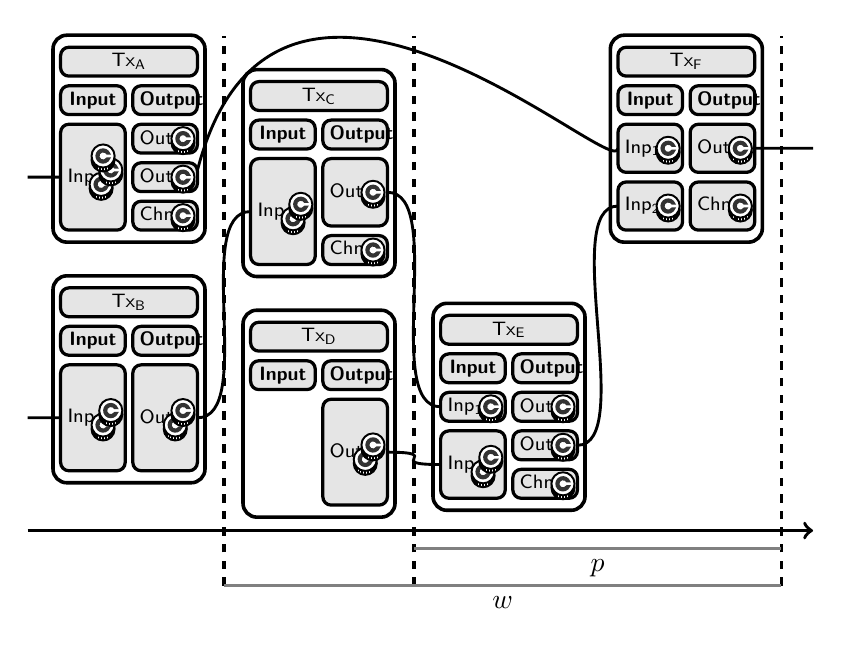
\begin{tikzpicture}
	\def \debugPoint   {}%
%b	\def \debugPoint   {point}%
	% font settings ############################################################
	\def \fontset      {\scriptsize\sffamily}
	% color definition #########################################################
	\def \colorOut     {black!100!white}
	\def \colorIn      {black!10!white}
	% arrow and line definitions ###############################################
	\def \lineW        {1.3pt}
	% width/height definition ##################################################
	\def \picW         {\linewidth*25.5/31}%
	\def \picH         {\paperheight*7.75/31}%
	\def \TH           {\picH*0.4}%picH*0.5*0.8
	
	\def \WBA          {\picW*11.50/31}
	\def \WLA          {\picW* 7.75/31}
	\def \WBB          {\picW* 4.00/31}
	\def \WLB          {\picW* 0.25/31}
	\def \WBC          {\picW* 3.50/31}
	\def \WBD          {\picW*10.50/31}
	\def \WLD          {\picW*14.25/31}
	% width/height nodes/boxes###################################################
	\def \BOH          {\picH* 0.35  }
	\def \BOW          {\picW* 6.0/31}
	
	% node positioning
	\def \BIPX         {\BOW*0.2375}
	
	% tikz styles################################################################
	\tikzstyle{lineIO} = [
		- ,
		line width = \lineW*0.8,
	]
	\tikzstyle{nodeOuter}   = [
		draw,
		rectangle,
		rounded corners=5pt,
		solid,
		line width = \lineW,
		black,
		inner sep = 0pt,
		outer sep = 0pt,
		text width = \BOW,
		minimum width = \BOW,
		minimum height = \BOH*1.075,
	]
	\tikzstyle{nodeInner}   = [
		draw,
		rectangle,
		rounded corners=3pt,
		solid,
		line width = \lineW*0.9,
		black,
		fill = \colorIn,
		inner sep = 0pt,
		outer sep = 0pt,
	]
	\tikzstyle{nodeInnerA}  = [
		nodeInner,
		align = center,
		text width = \BOW*0.9-3pt,
		minimum width = \BOW*0.9,
		minimum height = \BOH*0.15,
	]
	\tikzstyle{nodeInnerB}  = [
		nodeInner,
		align = left,
		text width = \BOW*0.425-5pt,
		minimum width = \BOW*0.425,
	]
	\tikzstyle{nodeInnerBA} = [
		nodeInnerB,
		minimum height = \BOH*0.15,
	]	
	\tikzstyle{nodeInnerBAC}b= [
		nodeInnerB,
		minimum height = \BOH*0.15,
		align = center,
	]
	\tikzstyle{nodeInnerBB} = [
		nodeInnerB,
		minimum height = \BOH*0.25,
	]
	\tikzstyle{nodeInnerBC} = [
		nodeInnerB,
		minimum height = \BOH*0.35,
	]
	\tikzstyle{nodeInnerBD} = [
		nodeInnerB,
		minimum height = \BOH*0.55,
	]
	% coordinates ###############################################################
	% 1 | 2 | 3 | 4 | 5 | 6 | 7 | 8 | 9 | 10 | 11 | 12 | 13 | 14 |
	% A | B | C | D | E | F | G | H | I |  J |  K |  L |  M |  N |
	
	\coordinate (cen)       at ($(0.0,0.0)   + ( 0.0       , 0.0         )$) (cen)   [\debugPoint];%
	
	\coordinate (PLU)       at ($(cen)       + (-\picW*0.5 , \picH*0.5   )$) (PLU)   [\debugPoint];%
	\coordinate (PLD)       at ($(cen)       + (-\picW*0.5 ,-\picH*0.5   )$) (PLD)   [\debugPoint];%
	\coordinate (PRU)       at ($(cen)       + ( \picW*0.5 , \picH*0.5   )$) (PRU)   [\debugPoint];%
	\coordinate (PRD)       at ($(cen)       + ( \picW*0.5 ,-\picH*0.5   )$) (PRD)   [\debugPoint];%
	
	
	\coordinate (TC)        at ($(cen)       + ( 0.0       ,-\TH         )$) (TC)    [\debugPoint];%
	\coordinate (TL)        at ($(TC)        + (-\picW*0.5 , 0.0         )$) (TL)    [\debugPoint];%
	\coordinate (TR)        at ($(TC)        + ( \picW*0.5 , 0.0         )$) (TR)    [\debugPoint];%
	
	\coordinate (BAC)       at ($(cen)       + (-\WBA      , 0.0         )$) (BAC)   [\debugPoint];%
	\coordinate (LAC)       at ($(cen)       + (-\WLA      , 0.0         )$) (LAC)   [\debugPoint];%
	\coordinate (BBC)       at ($(cen)       + (-\WBB      , 0.0         )$) (BBC)   [\debugPoint];%
	\coordinate (LBC)       at ($(cen)       + (-\WLB      , 0.0         )$) (LBC)   [\debugPoint];%
	\coordinate (LDC)       at ($(cen)       + ( \WLD      , 0.0         )$) (LDC)   [\debugPoint];%
	\coordinate (BCC)       at ($(cen)       + ( \WBC      , 0.0         )$) (BCC)   [\debugPoint];%
	\coordinate (BDC)       at ($(cen)       + ( \WBD      , 0.0         )$) (BDC)   [\debugPoint];%
	
	\coordinate (LAD)       at ($(LAC)       + ( 0.0       ,-\picH*0.5   )$) (LAD)   [\debugPoint];%
	\coordinate (LAU)       at ($(LAC)       + ( 0.0       , \picH*0.5   )$) (LAU)   [\debugPoint];%
	\coordinate (LBD)       at ($(LBC)       + ( 0.0       ,-\picH*0.5   )$) (LBD)   [\debugPoint];%
	\coordinate (LBDA)      at ($(LBC)       + ( 0.0       ,-\picH*0.4325)$) (LBDA)  [\debugPoint];%
	\coordinate (LBU)       at ($(LBC)       + ( 0.0       , \picH*0.5   )$) (LBU)   [\debugPoint];%
	\coordinate (LCD)       at ($(LDC)       + ( 0.0       ,-\picH*0.5   )$) (LCD)   [\debugPoint];%
	\coordinate (LCDA)      at ($(LDC)       + ( 0.0       ,-\picH*0.4325)$) (LCDA)  [\debugPoint];%
	\coordinate (LCU)       at ($(LDC)       + ( 0.0       , \picH*0.5   )$) (LCU)   [\debugPoint];%
	%coordinates, Box A Down, Tx_B		
	\coordinate (BADCC)     at ($(BAC)       + ( 0.0       ,-\picH*0.125 )$) (BADCC) [\debugPoint];%
	\coordinate (BADCL)     at ($(BADCC)     + (-\BIPX     , 0.0         )$) (BADCL) [\debugPoint];%
	\coordinate (BADCR)     at ($(BADCC)     + ( \BIPX     , 0.0         )$) (BADCR) [\debugPoint];%
	\coordinate (BADAC)     at ($(BADCC)     + ( 0.0       ,-\BOH *0.4   )$) (BADAC) [\debugPoint];%
	\coordinate (BADAL)     at ($(BADAC)     + (-\BIPX     , 0.0         )$) (BADAL) [\debugPoint];%
	\coordinate (BADAR)     at ($(BADAC)     + ( \BIPX     , 0.0         )$) (BADAR) [\debugPoint];%
	\coordinate (BADBC)     at ($(BADCC)     + ( 0.0       ,-\BOH *0.2   )$) (BADBC) [\debugPoint];%
	\coordinate (BADBL)     at ($(BADBC)     + (-\BIPX     , 0.0         )$) (BADBL) [\debugPoint];%
	\coordinate (BADBR)     at ($(BADBC)     + ( \BIPX     , 0.0         )$) (BADBR) [\debugPoint];%
	\coordinate (BADDC)     at ($(BADCC)     + ( 0.0       , \BOH *0.2   )$) (BADDC) [\debugPoint];%
	\coordinate (BADDL)     at ($(BADDC)     + (-\BIPX     , 0.0         )$) (BADDL) [\debugPoint];%
	\coordinate (BADDR)     at ($(BADDC)     + ( \BIPX     , 0.0         )$) (BADDR) [\debugPoint];%
	\coordinate (BADEC)     at ($(BADCC)     + ( 0.0       , \BOH *0.4   )$) (BADEC) [\debugPoint];%	
	%coordinates, Box A Up, Tx_A
	\coordinate (BAUCC)     at ($(BAC)       + ( 0.0       , \picH*0.3125)$) (BAUCC) [\debugPoint];%
	\coordinate (BAUCL)     at ($(BAUCC)     + (-\BIPX     , 0.0         )$) (BAUCL) [\debugPoint];%
	\coordinate (BAUCR)     at ($(BAUCC)     + ( \BIPX     , 0.0         )$) (BAUCR) [\debugPoint];%
	\coordinate (BAUAC)     at ($(BAUCC)     + ( 0.0       ,-\BOH *0.4   )$) (BAUAC) [\debugPoint];%
	\coordinate (BAUAL)     at ($(BAUAC)     + (-\BIPX     , 0.0         )$) (BAUAL) [\debugPoint];%
	\coordinate (BAUAR)     at ($(BAUAC)     + ( \BIPX     , 0.0         )$) (BAUAR) [\debugPoint];%
	\coordinate (BAUBC)     at ($(BAUCC)     + ( 0.0       ,-\BOH *0.2   )$) (BAUBC) [\debugPoint];%
	\coordinate (BAUBL)     at ($(BAUBC)     + (-\BIPX     , 0.0         )$) (BAUBL) [\debugPoint];%
	\coordinate (BAUBR)     at ($(BAUBC)     + ( \BIPX     , 0.0         )$) (BAUBR) [\debugPoint];%
	\coordinate (BAUDC)     at ($(BAUCC)     + ( 0.0       , \BOH *0.2   )$) (BAUDC) [\debugPoint];%
	\coordinate (BAUDL)     at ($(BAUDC)     + (-\BIPX     , 0.0         )$) (BAUDL) [\debugPoint];%
	\coordinate (BAUDR)     at ($(BAUDC)     + ( \BIPX     , 0.0         )$) (BAUDR) [\debugPoint];%
	\coordinate (BAUEC)     at ($(BAUCC)     + ( 0.0       , \BOH *0.4   )$) (BAUEC) [\debugPoint];%
	%coordinates, Box B Down, Tx_D	
	\coordinate (BBDCC)     at ($(BBC)       + ( 0.0       ,-\picH*0.1875)$) (BBDCC) [\debugPoint];%	
	\coordinate (BBDCL)     at ($(BBDCC)     + (-\BIPX     , 0.0         )$) (BBDCL) [\debugPoint];%
	\coordinate (BBDCR)     at ($(BBDCC)     + ( \BIPX     , 0.0         )$) (BBDCR) [\debugPoint];%
	\coordinate (BBDAC)     at ($(BBDCC)     + ( 0.0       ,-\BOH *0.4   )$) (BBDAC) [\debugPoint];%
	\coordinate (BBDAL)     at ($(BBDAC)     + (-\BIPX     , 0.0         )$) (BBDAL) [\debugPoint];%
	\coordinate (BBDAR)     at ($(BBDAC)     + ( \BIPX     , 0.0         )$) (BBDAR) [\debugPoint];%
	\coordinate (BBDBC)     at ($(BBDCC)     + ( 0.0       ,-\BOH *0.2   )$) (BBDBC) [\debugPoint];%
	\coordinate (BBDBL)     at ($(BBDBC)     + (-\BIPX     , 0.0         )$) (BBDBL) [\debugPoint];%
	\coordinate (BBDBR)     at ($(BBDBC)     + ( \BIPX     , 0.0         )$) (BBDBR) [\debugPoint];%
	\coordinate (BBDDC)     at ($(BBDCC)     + ( 0.0       , \BOH *0.2   )$) (BBDDC) [\debugPoint];%
	\coordinate (BBDDL)     at ($(BBDDC)     + (-\BIPX     , 0.0         )$) (BBDDL) [\debugPoint];%
	\coordinate (BBDDR)     at ($(BBDDC)     + ( \BIPX     , 0.0         )$) (BBDDR) [\debugPoint];%
	\coordinate (BBDEC)     at ($(BBDCC)     + ( 0.0       , \BOH *0.4   )$) (BBDEC) [\debugPoint];%
	%coordinates, Box B Up, Tx_C
	\coordinate (BBUCC)     at ($(BBC)       + ( 0.0       , \picH*0.2500)$) (BBUCC) [\debugPoint];%	
	\coordinate (BBUCL)     at ($(BBUCC)     + (-\BIPX     , 0.0         )$) (BBUCL) [\debugPoint];%
	\coordinate (BBUCR)     at ($(BBUCC)     + ( \BIPX     , 0.0         )$) (BBUCR) [\debugPoint];%
	\coordinate (BBUAC)     at ($(BBUCC)     + ( 0.0       ,-\BOH *0.4   )$) (BBUAC) [\debugPoint];%
	\coordinate (BBUAL)     at ($(BBUAC)     + (-\BIPX     , 0.0         )$) (BBUAL) [\debugPoint];%
	\coordinate (BBUAR)     at ($(BBUAC)     + ( \BIPX     , 0.0         )$) (BBUAR) [\debugPoint];%
	\coordinate (BBUBC)     at ($(BBUCC)     + ( 0.0       ,-\BOH *0.2   )$) (BBUBC) [\debugPoint];%
	\coordinate (BBUBL)     at ($(BBUBC)     + (-\BIPX     , 0.0         )$) (BBUBL) [\debugPoint];%
	\coordinate (BBUBR)     at ($(BBUBC)     + ( \BIPX     , 0.0         )$) (BBUBR) [\debugPoint];%
	\coordinate (BBUDC)     at ($(BBUCC)     + ( 0.0       , \BOH *0.2   )$) (BBUDC) [\debugPoint];%
	\coordinate (BBUDL)     at ($(BBUDC)     + (-\BIPX     , 0.0         )$) (BBUDL) [\debugPoint];%
	\coordinate (BBUDR)     at ($(BBUDC)     + ( \BIPX     , 0.0         )$) (BBUDR) [\debugPoint];%
	\coordinate (BBUEC)     at ($(BBUCC)     + ( 0.0       , \BOH *0.4   )$) (BBUEC) [\debugPoint];%
	%coordinates, Box C Down, Tx_E	
	\coordinate (BCDCC)     at ($(BCC)       + ( 0.0       ,-\picH*0.175 )$) (BCDCC) [\debugPoint];%	
	\coordinate (BCDCL)     at ($(BCDCC)     + (-\BIPX     , 0.0         )$) (BCDCL) [\debugPoint];%
	\coordinate (BCDCR)     at ($(BCDCC)     + ( \BIPX     , 0.0         )$) (BCDCR) [\debugPoint];%
	\coordinate (BCDAC)     at ($(BCDCC)     + ( 0.0       ,-\BOH *0.4   )$) (BCDAC) [\debugPoint];%
	\coordinate (BCDAL)     at ($(BCDAC)     + (-\BIPX     , 0.0         )$) (BCDAL) [\debugPoint];%
	\coordinate (BCDAR)     at ($(BCDAC)     + ( \BIPX     , 0.0         )$) (BCDAR) [\debugPoint];%
	\coordinate (BCDBC)     at ($(BCDCC)     + ( 0.0       ,-\BOH *0.2   )$) (BCDBC) [\debugPoint];%
	\coordinate (BCDBL)     at ($(BCDBC)     + (-\BIPX     , 0.0         )$) (BCDBL) [\debugPoint];%
	\coordinate (BCDBR)     at ($(BCDBC)     + ( \BIPX     , 0.0         )$) (BCDBR) [\debugPoint];%
	\coordinate (BCDDC)     at ($(BCDCC)     + ( 0.0       , \BOH *0.2   )$) (BCDDC) [\debugPoint];%
	\coordinate (BCDDL)     at ($(BCDDC)     + (-\BIPX     , 0.0         )$) (BCDDL) [\debugPoint];%
	\coordinate (BCDDR)     at ($(BCDDC)     + ( \BIPX     , 0.0         )$) (BCDDR) [\debugPoint];%
	\coordinate (BCDEC)     at ($(BCDCC)     + ( 0.0       , \BOH *0.4   )$) (BCDEC) [\debugPoint];%
	%coordinates, Box D Up, Tx_F
	\coordinate (BDUCC)     at ($(BDC)       + ( 0.0       , \picH*0.3125)$) (BDUCC) [\debugPoint];%	
	\coordinate (BDUCL)     at ($(BDUCC)     + (-\BIPX     , 0.0         )$) (BDUCL) [\debugPoint];%
	\coordinate (BDUCR)     at ($(BDUCC)     + ( \BIPX     , 0.0         )$) (BDUCR) [\debugPoint];%
	\coordinate (BDUAC)     at ($(BDUCC)     + ( 0.0       ,-\BOH *0.4   )$) (BDUAC) [\debugPoint];%
	\coordinate (BDUAL)     at ($(BDUAC)     + (-\BIPX     , 0.0         )$) (BDUAL) [\debugPoint];%
	\coordinate (BDUAR)     at ($(BDUAC)     + ( \BIPX     , 0.0         )$) (BDUAR) [\debugPoint];%
	\coordinate (BDUBC)     at ($(BDUCC)     + ( 0.0       ,-\BOH *0.2   )$) (BDUBC) [\debugPoint];%
	\coordinate (BDUBL)     at ($(BDUBC)     + (-\BIPX     , 0.0         )$) (BDUBL) [\debugPoint];%
	\coordinate (BDUBR)     at ($(BDUBC)     + ( \BIPX     , 0.0         )$) (BDUBR) [\debugPoint];%
	\coordinate (BDUDC)     at ($(BDUCC)     + ( 0.0       , \BOH *0.2   )$) (BDUDC) [\debugPoint];%
	\coordinate (BDUDL)     at ($(BDUDC)     + (-\BIPX     , 0.0         )$) (BDUDL) [\debugPoint];%
	\coordinate (BDUDR)     at ($(BDUDC)     + ( \BIPX     , 0.0         )$) (BDUDR) [\debugPoint];%
	\coordinate (BDUEC)     at ($(BDUCC)     + ( 0.0       , \BOH *0.4   )$) (BDUEC) [\debugPoint];%
	
	\coordinate (INPD)      at ($(cen)       + (-\picW*0.5 ,-\picH*0.195 )$) (INPD)  [\debugPoint];%
	\coordinate (INPU)      at ($(cen)       + (-\picW*0.5 , \picH*0.2425)$) (INPU)  [\debugPoint];%
	\coordinate (OUTU)      at ($(cen)       + ( \picW*0.5 , \picH*0.2950)$) (OUTU)  [\debugPoint];%
	
	%clipping
	\clip ($(PLD) + ( 0.0 ,-0.5)$) rectangle ($(PRU) + ( 0.0 , 0.1)$);
	%basic picture
	
	\draw[ ->, solid , line width = \lineW] (TL)   -- (TR);
	\draw[ - , dashed, line width = \lineW] (LAD)  -- (LAU);
	\draw[ - , dashed, line width = \lineW] (LBD)  -- (LBU);
	\draw[ - , dashed, line width = \lineW] (LCD)  -- (LCU);
	\draw[ - , gray  , line width = \lineW] (LBDA) -- node[midway, below, black]{$p$} (LCDA);
	\draw[ - , gray  , line width = \lineW] (LAD)  -- node[midway, below, black]{$w$} (LCD);
	%Nodes
	%node A Up, Tx_A
	\node[nodeOuter]   (NBAU)   at (BAUCC) {};	
	\node[nodeInnerA]  (NBAUEC) at (BAUEC) {\fontset{}$\mathsf{Tx_A}$};	
	\node[nodeInnerBAC](NBAUDL) at (BAUDL) {\fontset{}\textbf{Input}};	
	\node[nodeInnerBAC](NBAUDR) at (BAUDR) {\fontset{}\textbf{Output}};	
	\node[nodeInnerBD] (NBAUBL) at (BAUBL) {\fontset{}$\mathsf{Inp_1}$};	
	\node[nodeInnerBA] (NBAUCR) at (BAUCR) {\fontset{}$\mathsf{Out_1}$};
	\node[nodeInnerBA] (NBAUBR) at (BAUBR) {\fontset{}$\mathsf{Out_2}$};
	\node[nodeInnerBA] (NBAUAR) at (BAUAR) {\fontset{}Chng};
	
	%node A Down, Tx_B
	\node[nodeOuter]   (NBAD)   at (BADCC) {};	
	\node[nodeInnerA]  (NBADEC) at (BADEC) {\fontset{}$\mathsf{Tx_B}$};	
	\node[nodeInnerBAC](NBADDL) at (BADDL) {\fontset{}\textbf{Input}};	
	\node[nodeInnerBAC](NBADDR) at (BADDR) {\fontset{}\textbf{Output}};	
	\node[nodeInnerBD] (NBADBL) at (BADBL) {\fontset{}$\mathsf{Inp_1}$};	
	\node[nodeInnerBD] (NBADBR) at (BADBR) {\fontset{}$\mathsf{Out_1}$};
	
	%node B Up, Tx_C
	\node[nodeOuter]   (NBBU)   at (BBUCC)                      {};	
	\node[nodeInnerA]  (NBBUEC) at (BBUEC)                      {\fontset{}$\mathsf{Tx_C}$};	
	\node[nodeInnerBAC](NBBUDL) at (BBUDL)                      {\fontset{}\textbf{Input}};	
	\node[nodeInnerBAC](NBBUDR) at (BBUDR)                      {\fontset{}\textbf{Output}};	
	\node[nodeInnerBD] (NBBUBL) at (BBUBL)                      {\fontset{}$\mathsf{Inp_1}$};	
	\node[nodeInnerBC] (NBBUCR) at ($(BBUCR)+(0.0,-\BOH*0.10)$) {\fontset{}$\mathsf{Out_1}$};
	\node[nodeInnerBA] (NBBUAR) at (BBUAR)                      {\fontset{}Chng};
	
	%node B Down, Tx_D
	\node[nodeOuter]   (NBBD)   at (BBDCC) {};	
	\node[nodeInnerA]  (NBBDEC) at (BBDEC) {\fontset{}$\mathsf{Tx_D}$};	
	\node[nodeInnerBAC](NBBDDL) at (BBDDL) {\fontset{}\textbf{Input}};	
	\node[nodeInnerBAC](NBBDDR) at (BBDDR) {\fontset{}\textbf{Output}};	
	\node[nodeInnerBD] (NBBDBR) at (BBDBR) {\fontset{}$\mathsf{Out_1}$};
	
	%node C Down, Tx_E
	\node[nodeOuter]   (NBCD)   at (BCDCC)                     {};	
	\node[nodeInnerA]  (NBCDEC) at (BCDEC)                     {\fontset{}$\mathsf{Tx_E}$};	
	\node[nodeInnerBAC](NBCDDL) at (BCDDL)                     {\fontset{}\textbf{Input}};	
	\node[nodeInnerBAC](NBCDDR) at (BCDDR)                     {\fontset{}\textbf{Output}};	
	\node[nodeInnerBA] (NBCDCL) at (BCDCL)                     {\fontset{}$\mathsf{Inp_1}$};	
	\node[nodeInnerBC] (NBCDBL) at ($(BCDBL)+(0.0,-\BOH*0.1)$) {\fontset{}$\mathsf{Inp_2}$};	
	\node[nodeInnerBA] (NBCDCR) at (BCDCR)                     {\fontset{}$\mathsf{Out_1}$};
	\node[nodeInnerBA] (NBCDBR) at (BCDBR)                     {\fontset{}$\mathsf{Out_2}$};
	\node[nodeInnerBA] (NBCDAR) at (BCDAR)                     {\fontset{}Chng};
	
	%node D Up, Tx_F
	\node[nodeOuter]   (NBDU)   at (BDUCC)                      {};	
	\node[nodeInnerA]  (NBDUEC) at (BDUEC)                      {\fontset{}$\mathsf{Tx_F}$};	
	\node[nodeInnerBAC](NBUUDL) at (BDUDL)                      {\fontset{}\textbf{Input}};	
	\node[nodeInnerBAC](NBDUDR) at (BDUDR)                      {\fontset{}\textbf{Output}};	
	\node[nodeInnerBB] (NBDUCL) at ($(BDUCL)+(0.0,-\BOH*0.05)$) {\fontset{}$\mathsf{Inp_1}$};
	\node[nodeInnerBB] (NBDUCR) at ($(BDUCR)+(0.0,-\BOH*0.05)$) {\fontset{}$\mathsf{Out_1}$};
	\node[nodeInnerBB] (NBDUAL) at ($(BDUAL)+(0.0, \BOH*0.05)$) {\fontset{}$\mathsf{Inp_2}$};
	\node[nodeInnerBB] (NBDUAR) at ($(BDUAR)+(0.0, \BOH*0.05)$) {\fontset{}Chng};
	
	%Arrows depending on nodes
	\draw[lineIO] (INPD)        .. controls ($(INPD)        + ( 0.00, 0.00)$) and ($(NBADBL.west) + ( 0.00, 0.00)$) .. (NBADBL.west);
	\draw[lineIO] (INPU)        .. controls ($(INPU)        + ( 0.00, 0.00)$) and ($(NBAUBL.west) + ( 0.00, 0.00)$) .. (NBAUBL.west);
	\draw[lineIO] (NBADBR.east) .. controls ($(NBADBR.east) + ( 0.75, 0.00)$) and ($(NBBUBL.west) + (-0.75, 0.00)$) .. (NBBUBL.west);
	\draw[lineIO] (NBAUBR.0012) .. controls ($(NBAUBR.east) + ( 1.00, 3.95)$) and ($(NBDUCL.west) + ( 0.00,-0.45)$) .. (NBDUCL.west);
	\draw[lineIO] (NBBDBR.east) .. controls ($(NBBDBR.east) + ( 0.75, 0.00)$) and ($(NBCDBL.west) + (-0.75, 0.00)$) .. (NBCDBL.west);
	\draw[lineIO] (NBBUCR.east) .. controls ($(NBBUCR.east) + ( 0.75, 0.00)$) and ($(NBCDCL.west) + (-0.75, 0.00)$) .. (NBCDCL.west);
	\draw[lineIO] (NBCDBR.east) .. controls ($(NBCDBR.east) + ( 0.75, 0.00)$) and ($(NBDUAL.west) + (-0.75, 0.00)$) .. (NBDUAL.west);
	\draw[lineIO] (NBDUCR.east) .. controls ($(NBDUCR.east) + ( 0.00, 0.00)$) and ($(OUTU)        + ( 0.00, 0.00)$) .. (OUTU);
	
	%Coin Symbols
	\pic[] () at ($(NBAUBL.east) + (-\BOH*0.125,-\BOH*0.0375)$) {coin={0.7pt}{0.05}{\BOH*0.12}};
	\pic[] () at ($(NBAUBL.east) + (-\BOH*0.075, \BOH*0.0375)$) {coin={0.7pt}{0.05}{\BOH*0.12}};
	\pic[] () at ($(NBAUBL.east) + (-\BOH*0.115, \BOH*0.1100)$) {coin={0.7pt}{0.05}{\BOH*0.12}};
	\pic[] () at ($(NBAUAR.east) + (-\BOH*0.075, 0.0        )$) {coin={0.7pt}{0.05}{\BOH*0.12}};
	\pic[] () at ($(NBAUBR.east) + (-\BOH*0.075, 0.0        )$) {coin={0.7pt}{0.05}{\BOH*0.12}};
	\pic[] () at ($(NBAUCR.east) + (-\BOH*0.075, 0.0        )$) {coin={0.7pt}{0.05}{\BOH*0.12}};
	
	\pic[] () at ($(NBADBL.east) + (-\BOH*0.115,-\BOH*0.0375)$) {coin={0.7pt}{0.05}{\BOH*0.12}};
	\pic[] () at ($(NBADBL.east) + (-\BOH*0.075, \BOH*0.0375)$) {coin={0.7pt}{0.05}{\BOH*0.12}};
	\pic[] () at ($(NBADBR.east) + (-\BOH*0.115,-\BOH*0.0375)$) {coin={0.7pt}{0.05}{\BOH*0.12}};
	\pic[] () at ($(NBADBR.east) + (-\BOH*0.075, \BOH*0.0375)$) {coin={0.7pt}{0.05}{\BOH*0.12}};
	
	\pic[] () at ($(NBBUBL.east) + (-\BOH*0.115,-\BOH*0.0375)$) {coin={0.7pt}{0.05}{\BOH*0.12}};
	\pic[] () at ($(NBBUBL.east) + (-\BOH*0.075, \BOH*0.0375)$) {coin={0.7pt}{0.05}{\BOH*0.12}};
	\pic[] () at ($(NBBUCR.east) + (-\BOH*0.075, 0.0        )$) {coin={0.7pt}{0.05}{\BOH*0.12}};
	\pic[] () at ($(NBBUAR.east) + (-\BOH*0.075, 0.0        )$) {coin={0.7pt}{0.05}{\BOH*0.12}};
	
	\pic[] () at ($(NBBDBR.east) + (-\BOH*0.115,-\BOH*0.0375)$) {coin={0.7pt}{0.05}{\BOH*0.12}};
	\pic[] () at ($(NBBDBR.east) + (-\BOH*0.075, \BOH*0.0375)$) {coin={0.7pt}{0.05}{\BOH*0.12}};
	
	\pic[] () at ($(NBCDCL.east) + (-\BOH*0.075, 0.0        )$) {coin={0.7pt}{0.05}{\BOH*0.12}};
	\pic[] () at ($(NBCDBL.east) + (-\BOH*0.115,-\BOH*0.0375)$) {coin={0.7pt}{0.05}{\BOH*0.12}};
	\pic[] () at ($(NBCDBL.east) + (-\BOH*0.075, \BOH*0.0375)$) {coin={0.7pt}{0.05}{\BOH*0.12}};
	\pic[] () at ($(NBCDAR.east) + (-\BOH*0.075, 0.0        )$) {coin={0.7pt}{0.05}{\BOH*0.12}};
	\pic[] () at ($(NBCDBR.east) + (-\BOH*0.075, 0.0        )$) {coin={0.7pt}{0.05}{\BOH*0.12}};
	\pic[] () at ($(NBCDCR.east) + (-\BOH*0.075, 0.0        )$) {coin={0.7pt}{0.05}{\BOH*0.12}};
	
	\pic[] () at ($(NBDUAL.east) + (-\BOH*0.075, 0.0        )$) {coin={0.7pt}{0.05}{\BOH*0.12}};
	\pic[] () at ($(NBDUCL.east) + (-\BOH*0.075, 0.0        )$) {coin={0.7pt}{0.05}{\BOH*0.12}};
	\pic[] () at ($(NBDUAR.east) + (-\BOH*0.075, 0.0        )$) {coin={0.7pt}{0.05}{\BOH*0.12}};
	\pic[] () at ($(NBDUCR.east) + (-\BOH*0.075, 0.0        )$) {coin={0.7pt}{0.05}{\BOH*0.12}};		
\end{tikzpicture} 